\let\negmedspace\undefined
\let\negthickspace\undefined
\documentclass[journal]{IEEEtran}
\usepackage[a5paper, margin=10mm, onecolumn]{geometry}
\usepackage{tfrupee} % Include tfrupee package

\setlength{\headheight}{1cm} % Set the height of the header box
\setlength{\headsep}{0mm}     % Set the distance between the header box and the top of the text

\usepackage{gvv-book}
\usepackage{gvv}
\usepackage{cite}
\usepackage{amsmath,amssymb,amsfonts,amsthm}
\usepackage{algorithmic}
\usepackage{graphicx}
\usepackage{textcomp}
\usepackage{xcolor}
\usepackage{txfonts}
\usepackage{listings}
\usepackage{enumitem}
\usepackage{mathtools}
\usepackage{gensymb}
\usepackage{comment}
\usepackage[breaklinks=true]{hyperref}
\usepackage{tkz-euclide} 
\usepackage{listings}
\def\inputGnumericTable{}                                 
\usepackage[latin1]{inputenc}                                
\usepackage{color}                                            
\usepackage{array}                                            
\usepackage{longtable}                                       
\usepackage{calc}                                             
\usepackage{multirow}                                         
\usepackage{hhline}                                           
\usepackage{ifthen}                                           
\usepackage{lscape}
\newcommand{\brak}[1]{\left( #1 \right)}
\usepackage{multicol}

% Marks the beginning of the document
\begin{document}
\bibliographystyle{IEEEtran}
\vspace{3cm}

\title{9.2.6}
\author{EE24BTECH11017 - D.Karthik}
{\let\newpage\relax\maketitle}
\renewcommand{\thefigure}{\theenumi}
\renewcommand{\thetable}{\theenumi}

\textbf{Exercise 9.2} In each of the Exercises 1 to 10 verify that the given functions (explicit or implicit) is a solution of the corresponding differential equation:
\begin{align}
    \text{Given Function: } y &= x \sin x\\
    \text{Differential Equation: } xy^{\prime} &= y + x\sqrt{x^2 - y^2},  \brak{x \neq 0, x > y \text{ or } x < -y}.
\end{align}

\subsection*{Theoretical Solution}

Rewriting the equation:
\begin{align}
y^{\prime} = \frac{y}{x} + \sqrt{x^2 - y^2}
\end{align}
We introduce a substitution to simplify the problem. Let:
\begin{align}
    y = x \sin \theta
\end{align}
where $\theta$ is a function of $x$. Then:
\begin{align}
    y^{\prime} = \frac{d}{dx}\brak{x \sin \theta} = \sin \theta + x \cos \theta \frac{d\theta}{dx}
    \end{align}

Substitute $y = x \sin \theta $ and $y^{\prime}$ into the differential equation:

\begin{align}
    x \sin\theta + x \cos\theta \frac{d\theta}{dx} = x \sin\theta + x \sqrt{x^2 - (x \sin\theta)^2}
\end{align}

Simplify the square root term:
\begin{align}
    x \sqrt{x^2 - (x \sin\theta)^2} = x \sqrt{x^2 (1 - \sin^2\theta)} = x^2 \cos\theta
\end{align}



Substitute this back into the equation:
\begin{align}
    x \sin\theta + x^2 \cos\theta \frac{d\theta}{dx} = x \sin\theta + x^2 \cos\theta
\end{align}


Cancel $x \brak{\sin\theta}$ from both sides:

\begin{align}
    x^2 \cos\theta \frac{d\theta}{dx} = x^2 \cos\theta
\end{align}

Divide through by $x^2 \cos\theta \brak{\text{valid as } x \neq 0 \text{ and } \cos\theta \neq 0}$:

\begin{align}
    \frac{d\theta}{dx} = 1
\end{align}

Integrate both sides:

\begin{align}
    \theta = x + C
\end{align}
where $C$ is the constant of integration.

Using the substitution $y = x \sin\theta$, we have:
\begin{align}
  y = x \sin(x + C) 
\end{align}
Thus, the general solution to the differential equation is:
\begin{align}
    y = x \sin\brak{x + C},  x \neq 0, \text{ and } x > y \text{ or } x < -y
\end{align}

\subsection*{Numerical Solution}
To numerically verify the solution, we use the Improved Euler's Method as follows:
Definition of derivative,
\begin{align}
    f^\prime(y) &\approx \lim_{h\to0}\frac{f(y+h)-f(y)}{h} \\
    f(y+h) &\approx f(y)+hf^\prime(y) \\
    \implies x_{n+1} &\approx x_{n} + h\frac{dx}{dy}\Big|_{x=x_{n}, y=y_{n}}
\end{align}

Difference equation,
\begin{align}
    y_{n+1} &\approx y_n + h \left( \frac{y_n}{x_n} + \sqrt{x_n^2 - y_n^2} \right), \quad x_{n+1} = x_n + h.
\end{align}

\begin{figure}[h]
    \centering
    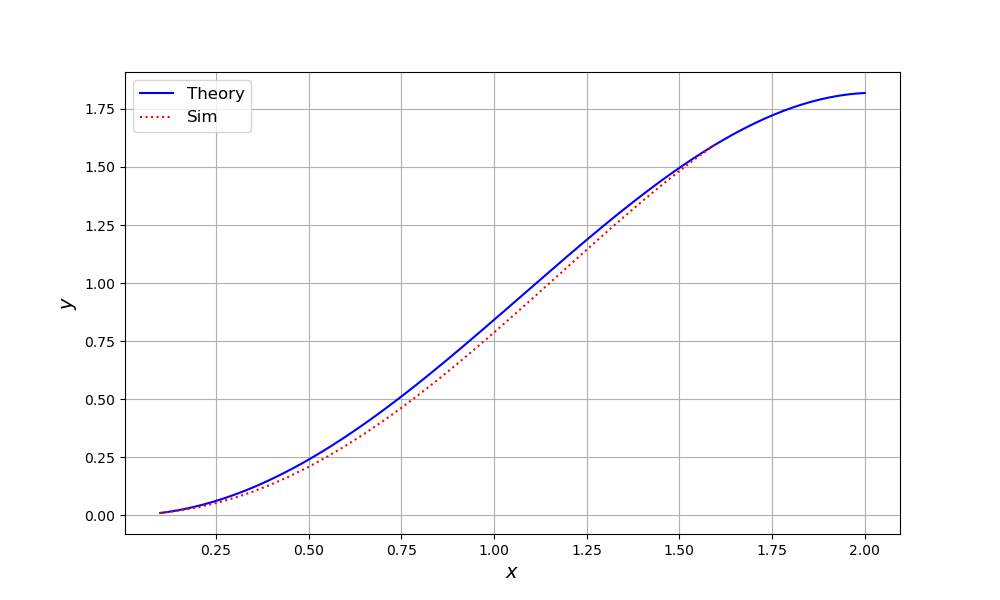
\includegraphics[width=\columnwidth]{figs/Figure_1.png}    
    \end{figure}
\end{document}

